\documentclass[10pt,UTF8]{ctexart}


\usepackage[margin=2cm,a4paper]{geometry}
%\usepackage[left=0.75in,top=0.6in,right=0.75in,bottom=1.0in,a4paper]{geometry}

\setmainfont{Caladea}
%% 也可以選用其它字庫:
% \setCJKmainfont[%
%   ItalicFont=AR PL KaitiM GB,
%   BoldFont=Noto Sans CJK SC,
% ]{Noto Serif CJK SC}
% \setCJKsansfont{Noto Sans CJK SC}
% \renewcommand{\kaishu}{\CJKfontspec{AR PL KaitiM GB}}

% 繁體中文
\setCJKmainfont[Path=fonts/ ]{NotoSansTC-Medium.otf}

\usepackage{minted}
\usepackage[breaklinks]{hyperref}

% Picture
% 導言區的此三行無變化
\usepackage{graphicx}
\usepackage{float} 
\usepackage{subfigure}
% 以下是新增的自定義格式更改
\usepackage[]{caption2} %新增調用的宏包
\renewcommand{\figurename}{Fig.} %重定義編號前綴詞
\renewcommand{\captionlabeldelim}{.~} %重定義分隔符
 %\roman 是羅馬數字編號,\alph是默認的字母編號,\arabic是阿拉伯數字編號,可按需替換下一行的相應位置
\renewcommand{\thesubfigure}{(\roman{subfigure})}%此外,還可設置圖編號顯示格式,加括號或者不加括號
\makeatletter \renewcommand{\@thesubfigure}{\thesubfigure \space}%子圖編號與名稱的間隔設置
\renewcommand{\p@subfigure}{} \makeatother

% Math
\usepackage {mathtools}
\usepackage{amssymb}

% Code
\usepackage{listings}
\usepackage{xcolor}
\lstset{
    % backgroundcolor=\color{red!50!green!50!blue!50},
    % 程式碼塊背景色為淺灰色
    rulesepcolor= \color{gray}, % 程式碼塊邊框顏色
    breaklines=true,  % 程式碼過長則換行
    numbers=left, % 行號在左側顯示
    numberstyle= \small,% 行號字型
    % eywordstyle= \color{red,% 關鍵字顏色
    commentstyle=\color{gray}, % 註釋顏色
    frame=shadowbox % 用方框框住程式碼塊
    }

\usepackage{hyperref}

\title{計算機視覺作業}
\author{干皓丞,2101212850, 信息工程學院}

\begin{document}
\maketitle


\section{作業目標與章節摘要}

對之前的論文清單做延伸,內容包括但不限於:論文內容、程式碼復現、實驗創新等,形成一份報告(原則上不多於 4 頁)。

\section{文章與作業狀況}

作業可以從 GitHub 下的 kancheng/kan-cs-report-in-2021 專案找到,作業程式碼與文件目錄為 kan-cs-report-in-2021/CV/cv-read-paper-work。實際執行的環境與實驗設備為 Google 的 Colab 、MacBook Pro (Retina, 15-inch, Mid 2014) 、 Acer Aspire R7 與 HP Victus (Nvidia GeForce RTX 3060)。該作業的論文清單為 CVPR 2021 Best Paper 中隨機挑出的 8 篇論文,將其全文進行概略上的翻譯,並嘗試論文清單中的幾篇論文,進行程式碼復現,而論文的全文翻譯可以於 kancheng/kan-readpaper-cv-and-ai-in-2021 的 CV 目錄下找到,當中的論文半數為 3D 領域的範疇,其領域如下。
\begin{figure}[H]
\centering 
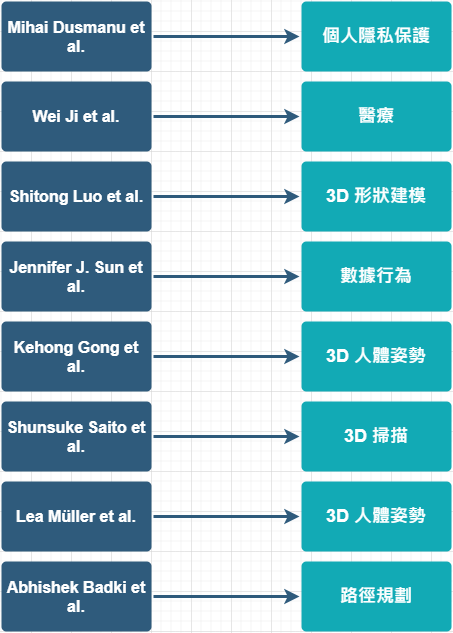
\includegraphics[width=0.50\textwidth]{m1.png} 
\caption{CVPR 2021 Best Paper - 8 篇}
\label{Test}
\end{figure}

\section{文章和摘要和貢獻}

1. 通過對抗仿射子空間嵌入保護隱私的圖像特徵

許多計算機視覺系統需要將使用者的圖像特徵上傳到雲端進行處理和儲存,而該研究發現可以利用這些特徵來恢復有關場景或主題的敏感資訊,比如通過重建原始圖像的外觀。而研究者們為了解決這個隱私問題,提出了一種新的隱私保護特徵表示。他們工作的核心思想是通過將每個特徵描述符去嵌入到包含原始特徵和對抗性特徵樣本的仿射子空間中,而後再進行刪除每個特徵描述符的約束。基於子空間到子空間距離的概念到啟用隱私保護的特徵是相互匹配的呈現。而研究者通過實驗證明了自己的方法的有效性及其與視覺定位和映射,跟人臉認證應用的高度實際相關性。前者與原始特徵相比,該研究的方法使對手恢復私人資訊得更加困難,相同的概念可以應用於其他領域,例如用於生物特徵認證的面部特徵。

\begin{figure}[H]
\centering 
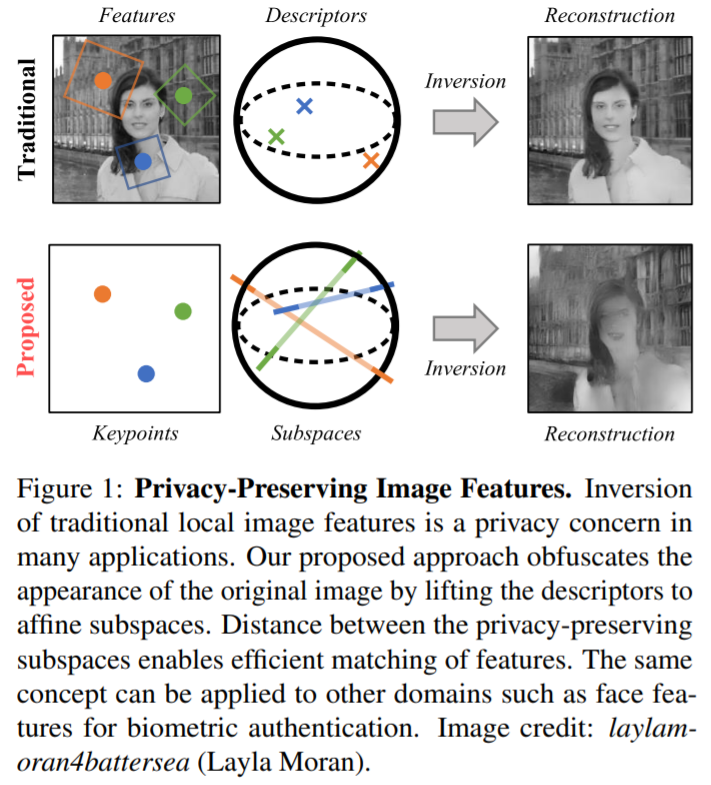
\includegraphics[width=0.50\textwidth]{r1.png} 
\caption{通過對抗仿射子空間嵌入保護隱私的圖像特徵}
\label{Test}
\end{figure}

2. 通過多評估者協議建模學習校準的醫學圖像分割

在醫學圖像分析領域中,通常會收集多個註釋,而每一個註釋都來自不同的臨床專家或評估者,以期望減少可能的診斷錯誤。而從計算機視覺的角度來看,採用通過多數票或來自首選評估者的簡單註釋來獲得的真實標籤已成為一種常見做法。當然此過程會忽略在原始多評估者註釋中根深蒂固的同意或不同意的等豐富資訊。研究者為了解決這個問題,他們建議對多評價者做一個名為 MR-Net 的 ex-plicitly model the multi-rater (dis-)agreement,此模型有兩個主要貢獻。首先,設計了一個專業知識推斷模塊或 EIM,將各個評分者的專業知識水平作為先驗知識嵌入,以形成高級語義的特徵。其次,研究者的方法能夠從粗略預測中重建多評分者的評分,並進一步利用多評分者中不一致的線索來提高分割性能,而此研究的工作是第一個進行在不同專業水平下為醫學圖像分割生成校準預測的研究,同時該研究在不同成像方式的五個醫學分割任務中進行了廣泛的實證實驗,證明 MRNet 對廣泛的醫學分割任務的有效性和適用性。

(1). 多評分者重建模塊 (MRM) 旨在根據專家先驗和模型的軟預測重建原始多評分者評分。通過利用融合軟標籤和原始多評級者註釋之間的內在相關性,這使得能夠估計反映評級者間可變性的不確定性圖。

(2). 為了更好地利用多評價者協議之間的豐富線索,我們進一步在我們的框架中加入了多評價者感知模塊(MPM),這在經驗上導致顯著的性能提升。

(3). 為了更好地利用多評價者的文字,我們進一步在我們的框架中加入了多評價者模塊(MPM),這在經驗上導致顯著的業績提升。

\begin{figure}[H]
\centering 
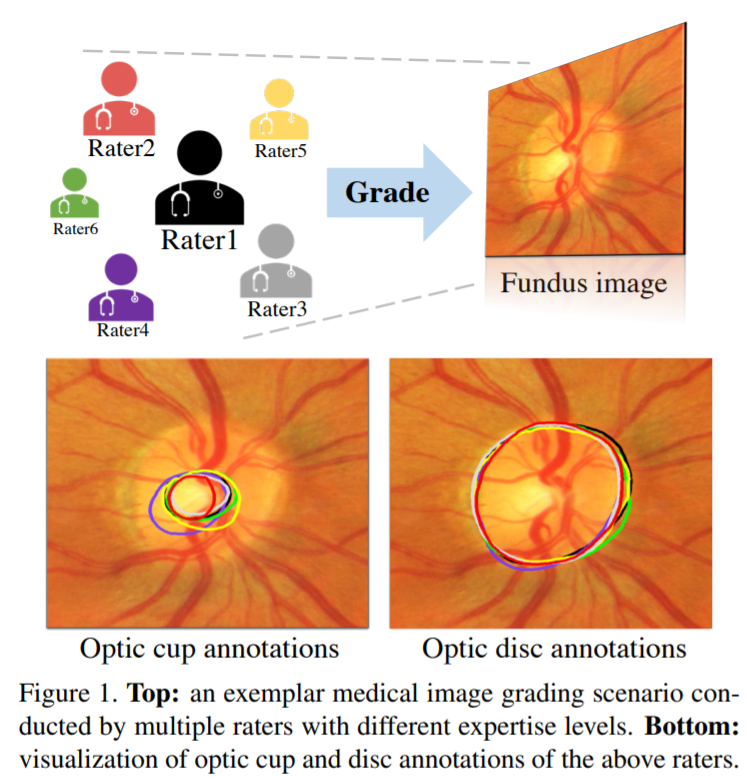
\includegraphics[width=0.50\textwidth]{r2.png} 
\caption{通過多評估者協議建模學習校準的醫學圖像分割}
\label{Test}
\end{figure}

3. 用於 3D 點雲生成的擴散概率模型

研究者提出了一個用於點雲生成的概率模型,該模型是各種 3D 視覺任務的基礎,比如形狀完成、上採樣、合成和數據增強。而受非平衡熱力學中擴散過程的啟發,我們將點雲中的點視為與熱浴接觸的熱力學系統中的粒子,它們從原始分佈擴散到噪聲分佈。因此,點雲生成相當於學習將噪聲分佈轉換為所需形狀分佈的反向擴散過程。具體來說,我們建議將點雲的反向擴散過程建模為以特定形狀為條件的馬爾可夫鏈。該研究推導出封閉形式的變分界用於訓練並提供模型的實現,而實驗結果表明,我們的模型在點雲生成和自動編碼方面取得了有競爭力的性能。其研究者的主要貢獻包括三點如下 :

(1). 研究者提出了一種新的點雲概率生成模型,其靈感來自非平衡熱力學中的擴散過程。

(2). 從以某種潛在形狀為條件的點雲可能性的變分下界得出一個易於處理的訓練目標。

(3). 大量實驗表明,該模型在點雲生成和自動編碼方面取得了有競爭力的性能。

\begin{figure}[H]
\centering 
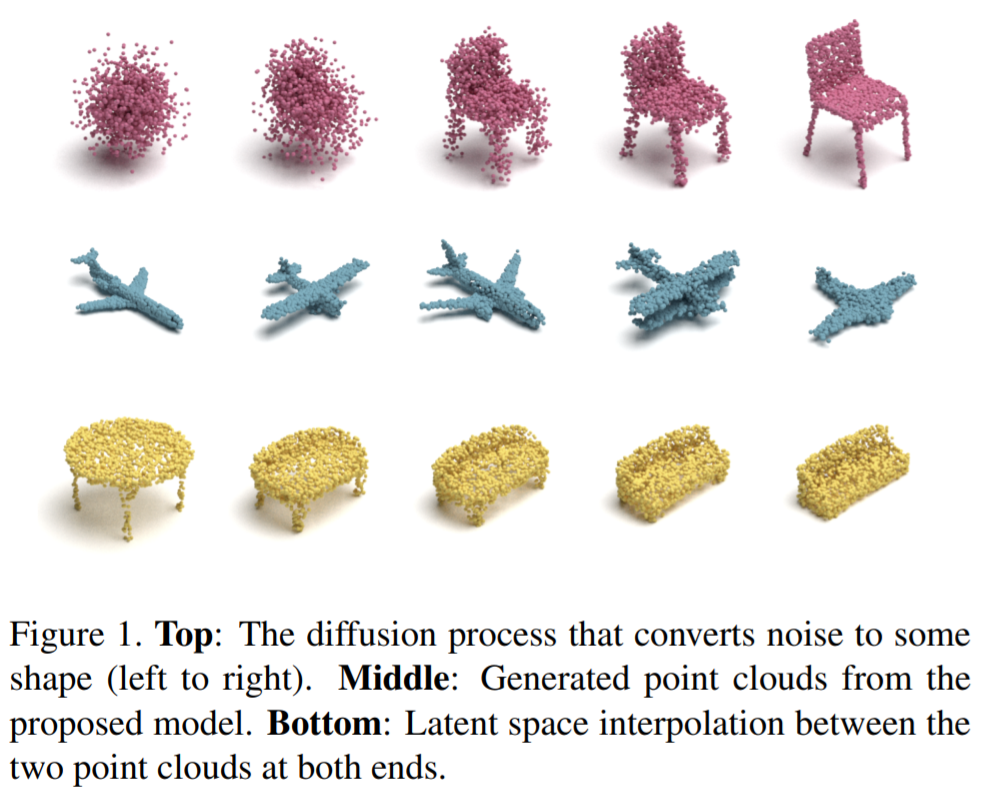
\includegraphics[width=0.50\textwidth]{r3.png} 
\caption{用於 3D 點雲生成的擴散概率模型}
\label{Test}
\end{figure}

4. 任務編程:學習數據高效行為表徵

%\begin{verbatim}
%
%\end{verbatim}

專業領域知識通常是準確註釋訓練集以進行深入分析所必需的,但從領域專家那裡獲取可能既繁瑣又耗時,該問題在自動化行為分析中尤為突出,其中從影片跟踪數據中檢測到 Agent 移動或者是感興趣的動作。為了減少註釋工作,研究者提出了 TREBA,一種基於多任務自監督學習學習註釋樣本有效軌跡嵌入以進行行為分析的方法。此方法中的任務可以由領域專家通過我們稱為“任務編程”的過程有效地設計,該過程使用程序對領域專家的結構化知識進行顯式編碼。通過為構建少量編程任務交換數據註釋時間,可以減少領域專家的總工作量。研究者使用來自行為神經科學的數據來去評估這種權衡,其中使用專門領域的知識來識別行為。該研究在兩個領域的三個資料集中展示了實驗結果:小鼠和果蠅。該研究的方法與最先進的特徵相比, TREBA 在不影響準確性的情況下將註釋負擔減少了 10 倍。而其研究的結果表明,任務編程和自我監督可以成為減少領域專家註釋工作的有效方法。

其主要貢獻三點如下:

(1). 研究者引入任務編程作為領域專家減少註釋工作和編碼結構知識的有效方式,並開發了一種使用自我監督和程序監督學習註釋樣本有效軌跡表示的新方法。

(2). 研究了任務編程、數據註釋和不同解碼器損失對行為分類器性能的影響。

(3). 我們在兩個領域中的三個資料集上演示了這些表示,表明該研究的方法可以導緻小鼠減少 10 個註釋,蒼蠅減少 2 個註釋。

\begin{figure}[H]
\centering 
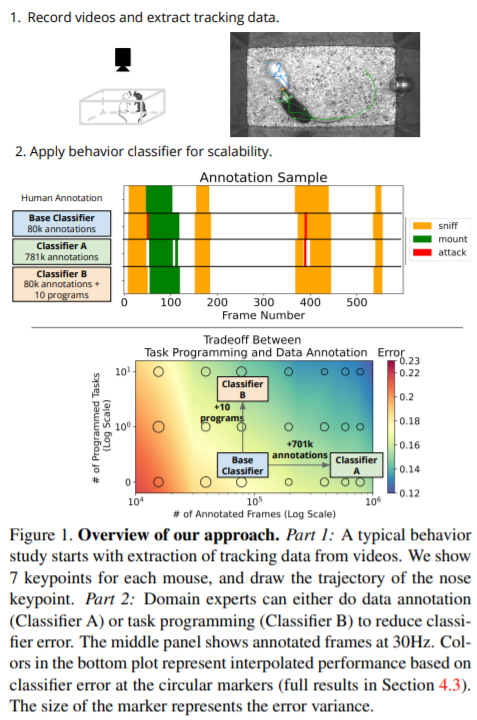
\includegraphics[width=0.50\textwidth]{r4.png} 
\caption{任務編程:學習數據高效行為表徵}
\label{Test}
\end{figure}

5. PoseAug:用於 3D 人體姿勢估計的可微姿勢增強框架

現有的 3D 人體姿態估計器對新數據集的泛化性能較差,這主要是由於訓練數據中 2D-3D 姿態對的多樣性有限。	而研究者為了解決這個問題,我們提出了 PoseAug,這是一種新的自動增強框架,它可以學習將可用的訓練姿勢增加到更大的多樣性,從而提高經過訓練的 2D 到 3D 姿勢估計器的泛化。

具體來說,PoseAug 引入了一種新穎的姿勢增強器,它可以通過可微分操作來學習調整姿勢的各種幾何因素,包含例人的姿勢、身體大小、視點和位置。而有了這種可區分的容量,增強器可以與 3D 姿態估計器聯合優化,並將估計誤差作為反饋,以在線方式生成更多樣和更難的姿態。此外,PoseAug 引入了一種新穎的部分感知運動鏈空間來評估局部關節角度的合理性,並相應地開發了一個判別模塊以確保增強姿勢的合理性。

這些精心設計的設計使 PoseAug 能夠生成比現有離線增強方法更多樣化但更合理的姿勢,從而更好地泛化姿勢估計器。而且PoseAug 是通用的,易於應用於各種 3D 姿勢估計器,在研究中大量實驗表明,PoseAug 在場景內和跨場景數據集上都帶來了明顯的改進。值得注意的是,它在跨資料集評估設置下在 MPI-INF-3DHP 上實現了 88.6% 的 3D PCK,比之前名為 EvoSkeleton (CVPR 2020) 的基於數據增強的最佳方法提高了 9.1%。該貢獻是三方面如下 :

(1). 該工作是第一個研究 3D 人體姿勢估計的可微數據增強的研究。

(2). 提出了一個可微的姿態增強器,連同誤差反饋設計,它生成多樣化和逼真的 2D-3D 姿態對來訓練 3D 姿態估計器,並在很大程度上增強了模型的泛化能力。

(3). 提出了一種新的部分感知 3D 鑑別器,它通過局部監督擴大了增強姿勢的可行區域,確保了數據的合理性和多樣性。

\begin{figure}[H]
\centering 
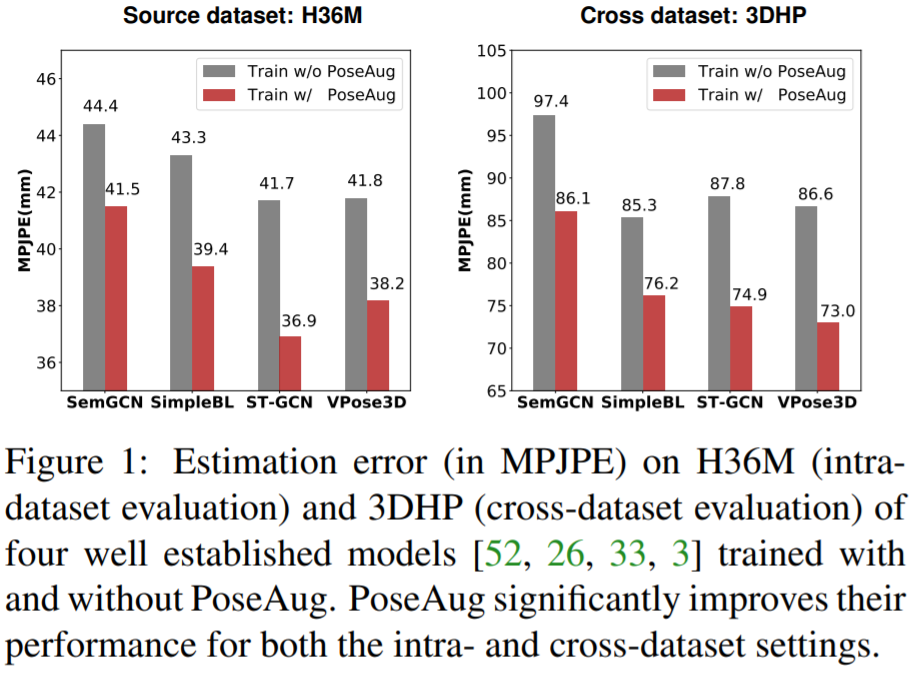
\includegraphics[width=0.50\textwidth]{r5.png} 
\caption{PoseAug:用於 3D 人體姿勢估計的可微姿勢增強框架}
\label{Test}
\end{figure}

6. SCANimate: Skinned Clothing Avatar Networks 的弱監督學習

該研究展示了名為 SCANimate 的一個端到端的可訓練框架,它可對一個穿著衣服的人進行原始 3D 掃描並將它們變成一個可動畫的化身,這些化身由姿勢參數驅動,並擁有可自然移動和變形的逼真服裝。SCANimate 不依賴於自定義網格模板 (a customized mesh template) 或表面網格註冊 (surface mesh registration)。該研究者們觀察到,將如 SMPL的參數化 3D 身體模型擬合到穿著衣服的人體掃描是容易處理的,而身體拓撲結構與掃描的表面配准通常則不然,因為衣服可能會顯著偏離身體形狀。

而研究還發現到鉸接變換是可逆的,從而導致擺姿勢和未擺姿勢的形狀的幾何循環一致性。這些觀察使研究者們找到了一種弱監督學習方法,該方法通過在沒有基於模板的表面配準的情況下解開鉸接變形來將掃描對齊到規範姿勢。此外,為了在對姿態相關變形建模的同時完成對齊掃描中的缺失區域,研究者們引入了一個局部姿態感知隱式函數,該函數學習使用學習的姿態校正來完成和建模幾何。此框架與常用的全局姿勢嵌入相比,我們的局部姿勢調節顯著降低了遠程虛假相關性,並提高了對未知姿勢的泛化能力,尤其是在訓練數據有限的情況下。 該研究的方法可以應用於姿態感知外觀建模以生成完全紋理化的頭像。研究者在具有不同訓練數據量的各種服裝類型上展示了 SCANimate 的方法,在每種設置的保真度和通用性方面均優於現有解決方案和其他變體。而主要貢獻如下 :

(1). 該框架為第一個端到端可訓練框架,用於從原始掃描構建高質量的參數化服裝人體模型,

(2). 一種具有幾何週期一致性的新型弱監督公式,可在不需要地面實況訓練數據的情況下將關節變形與局部姿態校正分開。

(3). 一種局部姿勢感知的隱式表面表示,它對依賴於姿勢的服裝變形進行建模並泛化到看不見的姿勢。

\begin{figure}[H]
\centering 
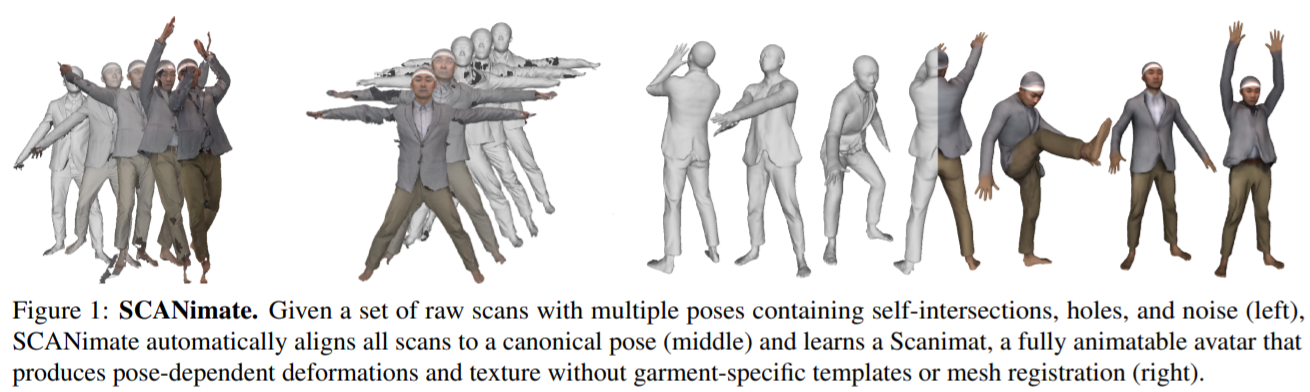
\includegraphics[width=0.50\textwidth]{r6.png} 
\caption{SCANimate: Skinned Clothing Avatar Networks 的弱監督學習}
\label{Test}
\end{figure}

7. 關於自我接觸和人體姿勢

人們每小時摸臉 23 次,他們交叉雙臂和雙腿,把手放在臀部等,雖然許多人的圖像包含某種形式的自我接觸,但當前的 3D 人體姿勢和形狀 (HPS) 回歸方法通常無法估計這種接觸,而為了解決這個問題,研究者開發了新的資料集和方法,通過自我接觸顯著改善人體姿勢估計。

首先,研究者創建了一個 3D 接觸姿勢 (3DCP) 數據集,其中包含適合 3D 掃描的 SMPL-X 身體以及來自 AMASS 的姿勢,我們對其進行改進以確保良好的接觸。其次,研究者利用它來創建通過 Amazon Mechanical Turk 收集的 Mimic-The-Pose (MTP) 圖像數據集,其中包含通過自我接觸模仿 3DCP 姿勢的人。其三,研究者開發了一種新穎的 HPS 優化方法 SMPLify-XMC,它包括接觸約束並在擬合期間使用已知的 3DCP 身體姿勢為 MTP 圖像創建接近真實的姿勢。第四,為了獲得更多的圖像多樣性,研究者使用離散自接觸 (DSC;  Discrete Self-Contact) 資訊標記野外圖像數據集,並使用另一種新的優化方法 SMPLify-DC,該方法在姿勢優化過程中利用離散接觸。最後,研究者在 SPIN 訓練期間使用自己的資料集來學習一個新的 3D 人體姿勢回歸器,稱為 TUCH (Towards Understanding Contact in Humans)。

該研究者們表明,新的自我接觸訓練資料顯著改善了對保留測試資料和現有資料集,比如 3DPW的 3D 人體姿勢估計。研究者的方法不僅改善了自接觸姿勢的結果,而且還提高了非接觸姿勢的準確性。而該研究主要貢獻六點如下:
 
(1). 研究者介紹了 TUCH,第一個用於自接觸姿勢的 HPS 回歸器,經過端到端訓練。

(2). 研究者創建了具有真實接觸 (3DCP) 的 3D 人體網格的新資料集。

(3). 研究者們定義了“模仿姿勢”MTP 任務和新的優化方法,以創建具有準確 3D 參考數據的野外圖像的新資料集。

(4). 創建了一個包含使用離散接觸標籤的參考姿勢的大型圖像資料集。

(5). 在實驗中表明,考慮自接觸信息可以通過兩種方式(數據和損失)改進姿勢估計,進而在 3D 姿勢估計基准上實現最先進的結果。

(6). 其資料和程式碼可用於研究目的。

\begin{figure}[H]
\centering 
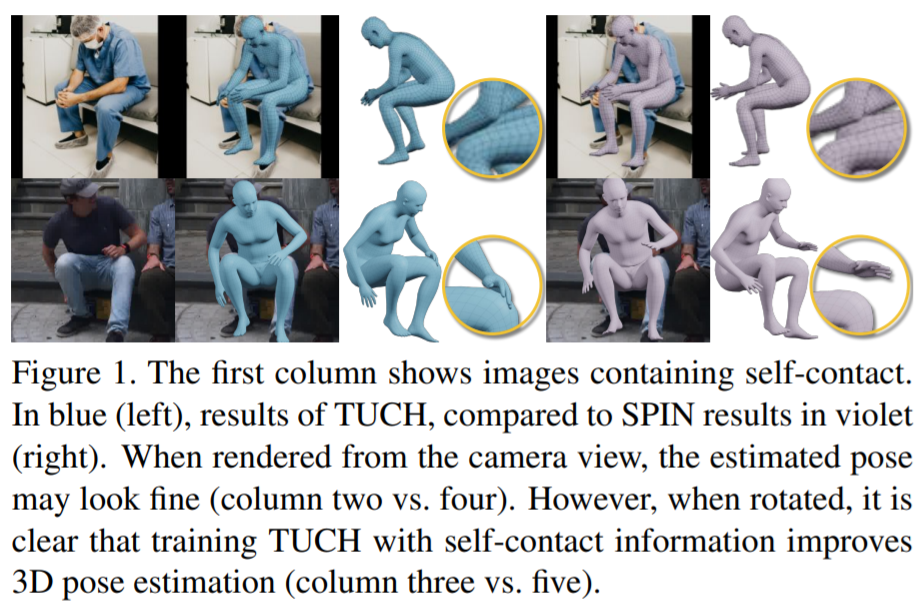
\includegraphics[width=0.50\textwidth]{r7.png} 
\caption{關於自我接觸和人體姿勢}
\label{Test}
\end{figure}

8. Binary TTC:自主導航的時間地理圍欄

接觸時間 (TTC),即物體與觀察者平面碰撞的時間,是路徑規劃的強大工具:它可能比場景中物體的深度、速度和加速度提供更多信息——即使對於人類也是如此。而 TTC 具有多種優勢,包括只需要一個單目、未校準的相機。然而,要做到回歸每個像素的 TTC 並不簡單,大多數現有方法對場景做出了過度簡化的假設。研究者們通過一系列更簡單的二元分類估計 TTC 來解決這一挑戰,他們以低延遲預測觀察者是否會在特定時間內與障礙物發生碰撞,這通常比知道精確的每像素 TTC 更重要。

對於這種情況,該研究的方法在 6.4 毫秒內提供了時間地理圍欄 (temporal geofence),此方法比現有方法快了 25 倍。當計算預算允許時,該研究的方法還可以通過任意精細的量化,包含連續值來估計每一個像素的 TTC。此方法是第一個以足夠高的幀速率提供 TTC 資訊 (binary or coarsely quantized) 以供實際使用的方法。

\begin{figure}[H]
\centering 
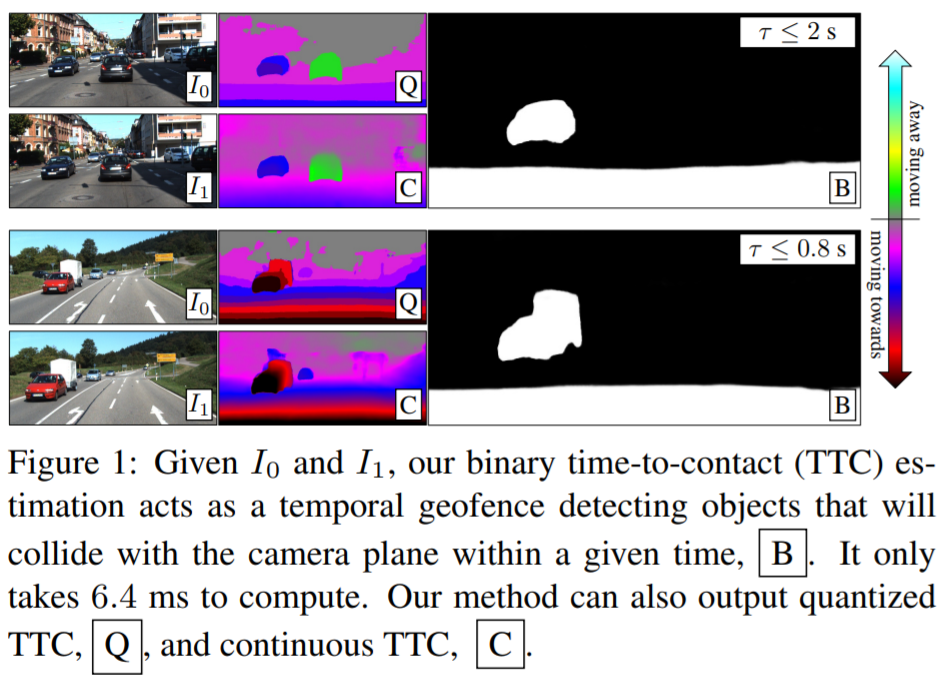
\includegraphics[width=0.50\textwidth]{r8.png} 
\caption{Binary TTC:自主導航的時間地理圍欄}
\label{Test}
\end{figure}

\section{參考文獻}

1. Mihai Dusmanu, Johannes L. Schönberger, Sudipta N. Sinha, Marc Pollefeys, 2021, "Privacy-Preserving Image Features via Adversarial Affine Subspace Embeddings", CVPR.

2. Wei Ji, Shuang Yu, Junde Wu, Kai Ma, Cheng Bian, Qi Bi, Jingjing Li, Hanruo Liu, Li Cheng, Yefeng Zheng, 2021, "Learning Calibrated Medical Image Segmentation via Multi-rater Agreement Modeling", CVPR.

3. Shitong Luo, Wei Hu, 2021, "Diffusion Probabilistic Models for 3D Point Cloud Generation", CVPR.

4. Jennifer J. Sun, Ann Kennedy, Eric Zhan, David J. Anderson, Yisong Yue, Pietro Perona, 2021, "Task Programming: Learning Data Efficient Behavior Representations", CVPR.

5. Kehong Gong, Jianfeng Zhang, Jiashi Feng, 2021, "PoseAug: A Differentiable Pose Augmentation Framework for 3D Human Pose Estimation", CVPR.

6. Shunsuke Saito, Jinlong Yang, Qianli Ma, Michael J. Black, 2021, "SCANimate: Weakly Supervised Learning of Skinned Clothed Avatar Networks", CVPR.

7. Lea Müller, Ahmed A. A. Osman, Siyu Tang, Chun-Hao P. Huang, Michael J. Black, 2021, "On Self-Contact and Human Pose", CVPR.

8. Abhishek Badki, Orazio Gallo, Jan Kautz, Pradeep Sen, 2021, "Binary TTC: A Temporal Geofence for Autonomous Navigation", CVPR.

\newpage

%\section{附錄}

% 數學意義說明

% $$\min \limits_{G}\max \limits_{D}{V_I(D,\ G)=V(D,G)-\lambda L_I(G,Q)}$$

%	\begin{lstlisting}[language={python}]

%	\end{lstlisting}

%\begin{enumerate}
%\item Y
%\item A
%\end{enumerate}

% \newpage

\clearpage

\end{document}